\subsection{The Hadoop Filesystem}
\label{sec:hdfs}
The Apache Hadoop Filesystem \cite{DBLP:conf/mss/ShvachkoKRC10}, or HDFS for short, is a scalable, distributed filesystem written in Java and originally developed for the Hadoop MapReduce computing framework.
Its design is heavily inspired by that of the Google File System (GFS) \cite{DBLP:conf/sosp/GhemawatGL03}.

The system is designed to handle very large files, typically several gigabytes to terabytes in size, by partitioning them in \emph{blocks} and storing the blocks on different machines.
To increase reliability, blocks are replicated multiple times, three by default, on different failure domains.
In a typical deployment, a block saved on a given machine will have another copy in the same rack and a final copy off-rack.
Due to the high storage cost of this replication scheme, HDFS 3.0 (set to be released at the end of 2017) optionally supports the use of erasure coding to lower the overhead while maintaining desirable retention characteristics.
Using either of the replication schemes effectively eliminates the need for RAID schemes on individual machines, as data retention is assured by the distributed filesystem itself.

Files in HDFS are expected to be accessed in a sequential fashion both during creation and during read operations and are considered mostly static.
The only modification allowed on a file is appending to the end and this operation can only be performed by one client at a time.
During read operations, the system supports the \texttt{seek} operation to read arbitrary portions of the file but it is a very inefficient operation that severely impacts throughput.

Clients interact with HDFS using a set of language-independent remote procedure call (RPC) endpoints.
The RPC system achieves language independence by using Protocol Buffers, a mechanism that allows the description of protocol messages and interactions (functions) in a high level language.
A protocol buffer specification, in the form of one or more \texttt{.proto} files, is compiled to target language code and then compiled (or interpreted) along with application files.
In HDFS, RPC is used both for communication between clients and the system and for communication within the system itself.

\subsubsection{Architecture}

\begin{figure}[ht]
\caption{HDFS components}
\label{fig:hdfs-block-diagram}
\centering
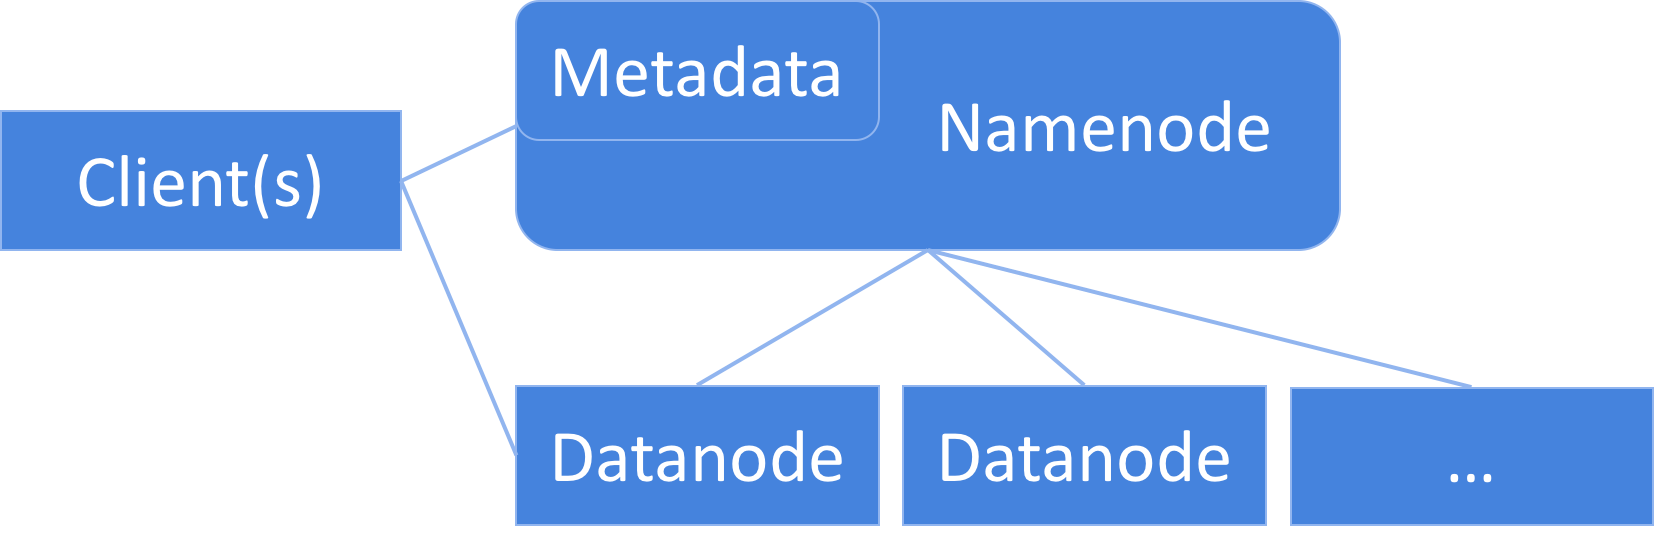
\includegraphics[width=1.0\textwidth]{images/hdfs-block-diagram.png}
\end{figure}

The HDFS system contains three main components, as shown in Figure \ref{fig:hdfs-block-diagram}:
\begin{enumerate}
\item one \emph{namenode}, with an optional hot standby copy,
\item a set of \emph{datanodes}, and
\item \emph{clients} interacting with the system.
\end{enumerate}

\paragraph{The namenode} is the central entity responsible for storing and applying modification to the system's metadata.
Metadata stored in the namenode includes information on the state and health of the cluster, information on how files are stored and replicated and finally information on the state of operations being executed.
Background threads in the namenode are also responsible for initiating periodic maintenance tasks such as block re-balancing and lease recovery.
It is a server application written in the Java programming language and it accepts commands from clients via the RPC interface mentioned above.
The namenode can also publish commands that will be executed by datanodes using the heartbeat mechanism.
The heartbeat mechanism is described in detail in Section \ref{sec:heartbeat}.
In HDFS the namenode is a single point of failure and, in the event of namenode failure, manual fail-over to a hot-standby is required to restore service availability.

\paragraph{Datanodes} are processes that handle physical storage of file blocks on disk.
A datanode is oblivious to the concept of file and only stores blocks.
To increase scalability, the datanode communicates directly with clients during read operations and with clients and other datanodes during write operations.
It also periodically reports its health and the integrity of the blocks it manages to the namenode via heartbeats.

\paragraph{Clients} are all programs that interact with the system to create, append or read files stored in the distributed file system.
As mentioned above, clients may be written in any language for which a protocol buffer implementation is available.
Depending on the operation type, client may interact with both namenode and datanodes to complete an operation.

While for some operations, such as listing the content of a directory, the client only performs a RPC call to the namenode, read and write operations require the client to contact both the namenode and datanodes.
HDFS follows a single-writer multiple-reader semantic for files, which means that there can be an arbitrarily large number of clients reading a file but only one writing data to it.

\subsubsection{Read pipeline}
When performing a read operation on a file, the client begins by contacting the namenode to get the addresses of the datanodes containing the first block of the file.
The list of datanodes holding a copy of the requested blocks is returned by the namenode sorted by proximity to the client requesting it according to the block placement policy.
The concept of proximity and how blocks are distributed onto datanodes is explained in Section \ref{sec:block-placement}.
The client then contacts the first datanodes to start reading the block.
If the connection to the datanode fails at any point during the operation, the client connects to the next datanode in the list and remembers the failed datanode so that it does not try to attempt a connection to it during following block reads.
If the checksum of the block read by the client is different from the expected one, the client communicates the checksum mismatch to the namenode before connecting to the next datanode in the list.
Once the client fully reads a block, it contacts the namenode to get the location of the next block and starts the process again.
In the actual implementation the client fetches several block locations with every call, further reducing the load on the namenode for client read operations.
It is worth mentioning that, on recent versions of Hadoop, the client can sometimes bypass the datanode completely and read the data directly from the local filesystem.
This operation is called a short-circuit local read.
The operation is only possible when the client is co-located on the same machine as the data-node housing the particular block requested, but this is often the case with data-aware frameworks such as MapReduce.

\subsubsection{Write pipeline}
\label{sec:write-pipeline}
Writes on HDFS are performed by one client at a time.
To maintain single-writer semantics, the client acquires a lease (essentially a lock) on every file it intends to write to.
The lease is periodically renewed by the client for as long as it is writing to the file.
If the lease is not renewed for a set amount of time, for instance because the client holding the lease crashed, it will expire.
There are two types of expiration times: soft, set at one minute and hard, set at 60 minutes.
When a lease expires after a soft timeout, it becomes available for other clients to claim through a procedure called \textit{lease recovery}.
On the other hand, when the hard limit for a lease expires, the namenode forcibly performs \textit{lease recovery} by closing the file, thereby making it available for new clients.
To decrease the network traffic generated by periodic lease renewal procedures on the namenode, a single lease renewal RPC call renews all the leases associated with the client performing the request.

Once the client acquires a lease, it contacts the namenode to get a new block id and a list of datanode to write data to.
The client will only write data and control messages such as \texttt{close}, to the first datanode which will then replicate the message to the second datanode in the list and so forth until there are no datanodes left.
Acknowledgments follow the same path in reverse, and are delivered in a single call to the client by the first datanode.
Finally, when the client closes the file, the lease is removed from the datanode and the block is closed by sending a close message through the pipeline.
The system is able to recover from failures during writing by performing \textit{pipeline recovery}.
Depending on the phase where the failure happens, the client can require a new set of datanodes from the namenode or exclude some of the datanodes from the pipeline.

\subsubsection{Block placement}
\label{sec:block-placement}
Apache HDFS stores a configurable number, three by default, of copies of each data block.
There are two primary reasons for this:
\begin{inparaenum}[i)]
\item to be able to withstand failure of a single data node holding the block and
\item to increase throughput by allowing different readers to read different copies of the same block
\end{inparaenum}.
To fulfill both purposes it is important to consider the placement of blocks in the context of the overall network topology where HDFS is deployed.
In a typical deployment, HDFS data nodes will be installed in server blades which will be installed in a rack.
Machines in a rack will be connected to the network via a TOR (top of the rack) switch, which will provide both connectivity between machines in the rack and connectivity to the other racks via a higher level switch.
This type of deployment assumes that inter-rack connections are lower latency and have more bandwidth, while intra-rack connections are more expensive both in terms of bandwidth and latency.
In this scenario, each rack represents a separate failure domain, as failure of the TOR switch, loss of connectivity to the higher level switch, or power failure effectively isolates all the machines in the rack from the network.
To avoid the scenario where the loss of a single rack compromises the availability of all the replicas of a block, HDFS distributes the replica of a block across racks, provided that the cluster operator provides the namenode with information on placement of datanodes.

As part of the setup for a write pipeline, the namenode provides the client with a ordered list of datanodes to write data to.
If datanode rack placements are configured in the namenode, datanodes are selected as follows:
\begin{itemize}
\item If the client is in the cluster, like a MapReduce job, and there is a datanode on the machine, the first block is placed on the same machine as the client.
\item If, on the other hand, the client is not part of the cluster, the first block is placed on a random node as there is no way to compute a distance metric between the client and the datanodes.
\item The second block is placed on a machine in a different rack than the first block.
\item The third block is placed on another machine on the same rack as the second machine.
\item The fourth block, if present, is placed on a different machine on the same rack as the first machine.
\item If any more blocks are present, they are randomly distributed.
\end{itemize}
This distribution scheme minimizes the amount of inter-rack transfers necessary to spread the blocks on more than one availability zone.

\subsubsection{Fault tolerance}
Apache HDFS is designed as a modern distributed system and as such, datanode failure is treated as a routine event and handled transparently without the need for manual intervention.
Datanodes periodically communicate their health status to the namenode by sending heartbeat messages.
When a datanode stops sending heartbeat messages, the namenode considers it failed, and therefore it regards all the blocks stored on it as not accessible to the cluster.

To maintain the correct number of replicas for every block the namenode runs a background thread called the \textit{replication monitor}.
The replication monitor periodically checks the number of replicas for every block in the system and performs remedial action if the number is lower or higher than required.
\begin{itemize}
\item In case the block is \textbf{over-replicated}, the replication monitor schedules the deletion of the excess replicas in such a way that the remaining copies still fulfill the block placement policy.
\item In case the block is \textbf{under-replicated}, for example as a result of datanode failure, the replication monitor schedules the creation of new replicas according to the block placement policy.
\end{itemize}

The operations scheduled by the replication monitors are executed by datanodes and are transmitted to the relevant datanodes via the heartbeat mechanism.

\subsubsection{Heartbeat}
\label{sec:heartbeat}
The mechanism used by the datanodes to communicate their status to the namenode is to send periodic heartbeat RPC messages to the namenode.
The interval of time between heartbeats can be specified in the configuration file of HDFS but by default it is three seconds.
Responses to heartbeat messages from namenode to datanodes also optionally contain commands for datanodes to execute, such as the deletion of blocks, the re-replication of a block to another datanode, and so forth.
The main advantage of delivering commands as responses to heartbeats instead of sending commands from the namenode to the datanodes is that it allows a single namenode to manage a far greater number of datanodes, removing a bottleneck to scalability.

\subsection{Scalability limitations of HDFS}
\label{sec:scalability-limitations}
A study conducted regarding the scalability limitations of HDFS \cite{shvachko2010hdfs} concluded that HDFS can manage an estimate 1 petabyte of data per gigabyte of metadata.
While Apache HDFS can be scaled to manage multi-petabyte clusters, its single-active namenode design effectively limits both the amount of metadata and the number of queries per second (QPS) a node can process, to the largest machine it can be installed on.
The amount of metadata is limited because they are stored as Java objects in the Java Virtual Machine (JVM) heap space, which is itself limited by the amount of main memory available in the machine.
Furthermore, Java objects have a 8 to 12 byte header which is used by the virtual machine, increasing the memory requirements even further.
The amount of QPS that the system can process is limited by both the number and speed of processors in the machine, the connection between clients (including datanodes) and the namenode itself, and the number of alterations that the system can apply to the metadata.
Metadata objects are, in principal, only altered in two ways: from periodic processing by the namenode and as a consequence of RPCs invoked by clients and datanodes.
Given that any number of these alterations can happen in parallel, the namenode protects the metadata with a global lock, the \textit{FSNamesystemLock}, which can be acquired by an arbitrary number of threads in \emph{read} mode, but requires exclusivity when acquired in \emph{write} mode.
All operations that require modification of the metadata are therefore executed serially, further lowering the amount of queries per second that the namenode can process.
Storing metadata in the JVM heap is also problematic due to increasingly long garbage collection pauses that freeze the entire process as the heap grows in size.

\clearpage